\documentclass{article}
\usepackage[utf8]{inputenc}
\usepackage{graphicx,float}

\title{Synthesis}
\author{Alex Booth\\ a.booth9@edu.salford.ac.uk}
\date{October 2022}

\begin{document}

\maketitle
\section{Abstract}
    \textit{Here goes the abstract}
\section{Introduction}
    Musical instruments have been part of human culture and craft since prehistory, playing a part in both written and verbal art, ceremony and celebration \cite{rault}.
    This report describes an attempted recreation using digital synthesis of two acoustic musical instruments from the western European musical tradition: A Mandolin and a flute.
    Acoustic musical instruments use an excited physical component to generate waves which are manipulated and shaped by the body or construction of the musical instrument. % CITE
    The generation of these waves, and their manipulation by the body of the musical instrument can be modelled using a series of oscillators, filters and modulators.
    Audio synthesis using analog circuitry was explored as soon as simple oscillators were readily available. Leading to instruments such as the theremin.  % WHEN?
    In order to emulate the sound of musical instruments, first we must understand the mathematical nature of sound as a signal.

    FM and additive synthesis methods are explored in this report.

\section{Theory}
    \subsection{Signal processing, generation and analysis}
        Any periodic continuous signal can be broken down into an infinite sum of weighted sines and cosines \cite{weisstein2004fourier}.
        A more generalised application of the Fourier series can be found in the Fourier transform, which in continuous time takes the form:
        \begin{equation}
            X(\omega) = \int_{-\infty}^{+\infty}x(t)e^{-j\omega t}dt
        \end{equation}
        However, as digital audio works in the discrete time domain, the integrals can be represented as sums and the Fourier series becomes:
        \begin{equation}
            X(\omega) = \sum_{-\infty}^{+\infty}x[n]e^{-j\omega t}dt
        \end{equation}
        In the 1960s, J.W. Cooley and John Tukey developed an algorithm to efficiently compute the discrete Fourier transform \cite{cooley1965algorithm}.
        This, and other discrete-time fourier transform algorithms became known as the fast Fourier transform(s) (FFT).
        MATLAB's in-built FFT function uses a more modern FFT algorithm from the the FFTW library \cite{frigo1998fftw}.
        Using a fourier transform, a complex sound can be broken down into it's frequency components.
        This allows the fundamental frequency and harmonics of the played note to be identified, due they will be the most prominent components of the frequency spectrum.
        However, the Fourier transform does not only show harmonic frequency content of a signal, it shows all frequency content of a signal.
        As such, any noise or other anharmonic frequency component, musical or not, will be shown on the transform.
        The simple inclusion of an observed frequency component may or may not be constructive to emulating the original played note.
        \\
        Musical synthesizers were first constructed to facilitate additive synthesis.
        This is where a series of oscillators generate basic waveforms such as sines, sawtooth and pulse waves.
        \begin{figure}[h]
            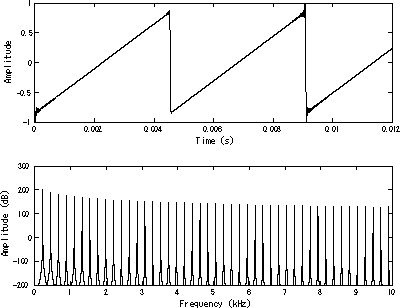
\includegraphics[scale=0.6]{images/Sawtooth.png}%
            \centering
            \caption{Waveform and frequency response of a sawtooth wave.}\cite{kraft2017lp}
        \end{figure}
        In the 1970s, FM synthesis was beginning to take form as a method of musical instrument emulation. Chowning's work outlined specific FM techniques for the emulation of various instruments \cite{chowning1973synthesis}.

    \subsection{Musical instruments}

\section{Methodology}
\section{Discussion}
\section{Conclusions}
\section{Appendix}
\subsection{Code}



\bibliographystyle{IEEEtran} % We choose the "plain" reference style
\bibliography{theBib.bib}

\end{document}


